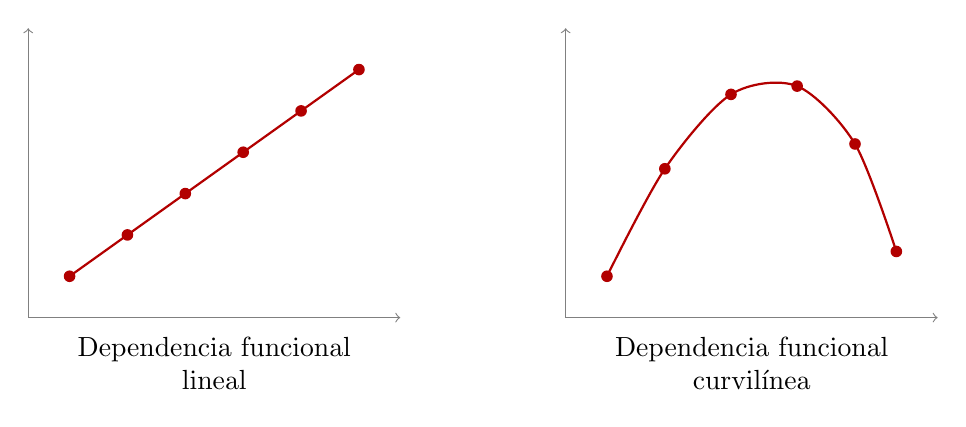
\begin{tikzpicture}[scale=1.05]
    % Dependencia lineal funcional
    \begin{scope}[xshift=1cm]
        \draw[->,gray] (0,0) -- (4.5,0);
        \draw[->,gray] (0,0) -- (0,3.5);
        \draw[red!70!black,thick] (0.5,0.5) -- (4,3.0);
        \foreach \x/\y in {0.5/0.5,1.2/1.0,1.9/1.5,2.6/2.0,3.3/2.5,4/3.0} {\fill[red!70!black] (\x,\y) circle (2pt);}
        \node[align=center] at (2.25,-0.55) {Dependencia funcional\\lineal};
    \end{scope}
    % Dependencia curvilínea funcional
    \begin{scope}[xshift=7.5cm]
        \draw[->,gray] (0,0) -- (4.5,0);
        \draw[->,gray] (0,0) -- (0,3.5);
        \draw[red!70!black,thick] plot[smooth] coordinates {(0.5,0.5) (1.2,1.8) (2.0,2.7) (2.8,2.8) (3.5,2.1) (4,0.8)};
        \foreach \x/\y in {0.5/0.5,1.2/1.8,2.0/2.7,2.8/2.8,3.5/2.1,4/0.8} {\fill[red!70!black] (\x,\y) circle (2pt);}
        \node[align=center] at (2.25,-0.55) {Dependencia funcional\\curvilínea};
    \end{scope}
\end{tikzpicture}